\textbf{Ejemplo 11}\\
Hallar el valor presente de 15 pagos que decrecen
linealmente en 400 COP, si el primer pago es de 5.000 COP y la tasa efectiva es del 4\% período año
vencido.\\ \\
%\newpage %USAR SOLO SI EL SOLUCIÓN QUEDA SOLO Y ES NECESARIO BAJARLO A LA SIGUIENTE PAGINA
\textbf{Solución.}\\
%La tabla ira centrada
\begin{center}
 \renewcommand{\arraystretch}{1.5}% Margenes de las celdas
 %Creación de la cuadricula de 3 columnas
 \begin{longtable}[H]{|p{0.333\linewidth}|p{0.3333\linewidth}|p{0.3333\linewidth}|}
  \hline
  \multicolumn{3}{|c|}{\cellcolor[HTML]{FFB183}\textbf{1. Declaración de variables}}                                                                                                                 \\ \hline
  \multicolumn{1}{|c|}{\cellcolor[HTML]{FFB183}\textbf{Variables monetarias}}                   & \multicolumn{1}{|c|}{\cellcolor[HTML]{FFB183}\textbf{Variables no monetarias}}                   & \multicolumn{1}{|c|}{\cellcolor[HTML]{FFB183}\textbf{Variables incógnitas}}                                                                         \\ \hline
  $R =  5{.}400 COP$  & $i=4,0\% \hspace{1mm} pav$ & $VP=? COP$                                                                                                                                                                            \\
  $L = 400 COP$  & $n=15 \hspace{1mm} pav$ & \\ \hline
  \multicolumn{3}{|c|}{\cellcolor[HTML]{FFB183}\textbf{2. Diagrama de flujo de caja}}                                                                                                                \\ \hline
  \multicolumn{3}{|p{\columnwidth}|}{
      \begin{center}
        \begin{tabular}{|c|c|}
          \hline
               Periodo (pav) & Flujo      \\ \hline
               	0             & \$   -    \\ \hline
                1             & \$ 500 \\ \hline
                2             & \$ 800 \\ \hline
                3             & \$ 1.200 \\ \hline
                4             & \$ 1.600 \\ \hline
                5             & \$ 2.000 \\ \hline
                6             & \$ 2.400 \\ \hline
                7             & \$ 2.800 \\ \hline
                8             & \$ 3.200 \\ \hline
                9             & \$ 3.600 \\ \hline
                10             & \$ 4.00 \\ \hline
                11             & \$ 4.400 \\ \hline
                12             & \$ 4.800 \\ \hline
                13             & \$ 5.200 \\ \hline
                14             & \$ 5.600 \\ \hline
                15             & \$ 6.000 \\ \hline
        \end{tabular}
      \end{center}
    } \\
  \multicolumn{3}{|c|}{\cellcolor[HTML]{FFB183}\textbf{3. Aplicación de funciones}}                                                                                                                  \\ \hline
  \multicolumn{3}{|p{\columnwidth}|}{Se aplicará la función valor presente VNA de la siguiente forma: \newline
  =VNA(0,04;J8::J22) con referencia en la hoja de
  Excel usada para el ejercicio.}                                                                                                                                                                    \\
  \multicolumn{3}{|c|}{ 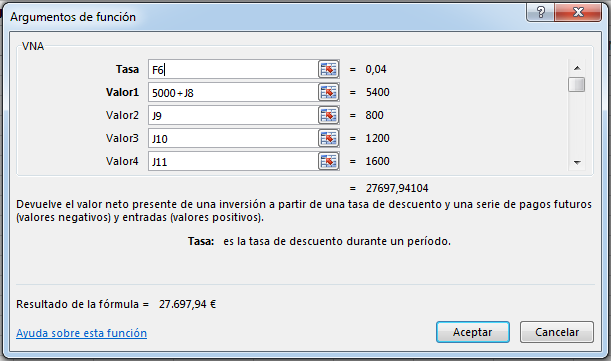
\includegraphics[trim=-5 -5 -5 -5 ,width=0.7\columnwidth]{11/excel1.png}}                                                                                                    \\ \hline
  \multicolumn{3}{|c|}{\cellcolor[HTML]{FFB183}\textbf{4. Gráfica}}                                                                                                                                  \\ \hline
  \multicolumn{3}{|c|}{ 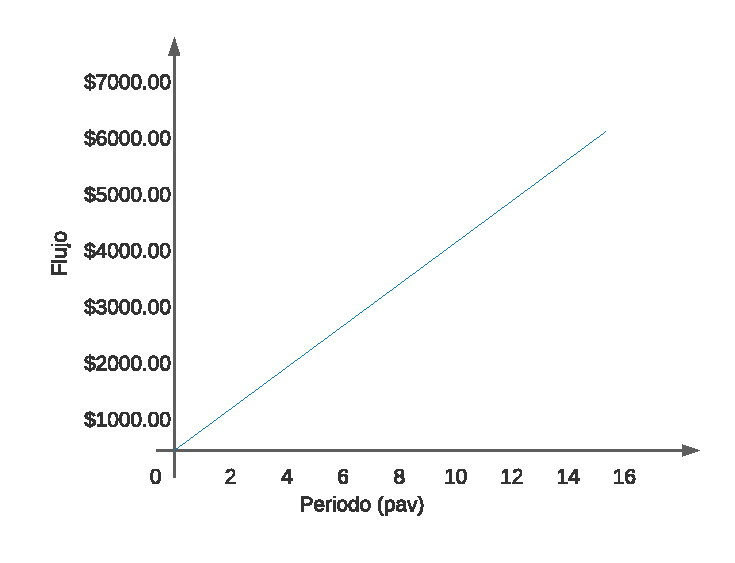
\includegraphics[trim=-5 -5 -5 -5 ,width=0.8\columnwidth]{11/gráfico.pdf}}                                                                                                   \\ \hline
  \multicolumn{3}{|c|}{\cellcolor[HTML]{FFB183}\textbf{5. Respuesta}}                                                                                                                                \\ \hline
  \multicolumn{3}{|c|}{El valor presente es VP =  COP 27.697,9410}                                                                                                                                      \\ \hline
 \end{longtable}
 %\newline \newline %USARLO SI CREES QUE ES NECESARIO
\end{center}
